%FilterDFE.tex
%
\documentclass[10pt,letterpaper,twoside,titlepage]{book}%
\title{DFE Filtering}
\author{MA~Laforge}%
\def\AMSFooterTag{MA Laforge: DFE Filtering}
\usepackage[singlespacing]{../Common/LaforgeDocStyle}%
%
\usepackage{graphicx}\graphicspath{{./figures/}}%
\usepackage{IEEEtrantools}%
\usepackage{amsmath}%
\usepackage{latexsym}%Provides the \Box command (for sheet resistance)
\usepackage[reim_shrthnd,reim_curly]{../Common/CustomCommands}%
\usepackage[sort,compress,noadjust]{cite}%Does not work for some reason
\usepackage{../Common/Hyphenation}%correct bad hyphenation here
%
%Custom commands:
%FilterDFE_CustCmds.tex
%Defines document-level custom commands
%
%Constants
%------------------------------------------------------------------------------
\newcommand{\maxfigwidth}{3.15in}%
%
%Equation alignment
%------------------------------------------------------------------------------
\newcommand{\EAtwocols}[4]{%
%Defines a 2-column line format for use in IEEEeqnarray.
%Output format:
%   [    #1][#2                 ][    #3][#4                 ]
%      w1        (1-w1)/2-w2        w2         (1-w1)/2
\parbox[t]{.15\linewidth}{\hfill\begin{IEEEeqnarraybox*}[][t]{r}#1\end{IEEEeqnarraybox*}}%
\parbox[t]{.35\linewidth}{\begin{IEEEeqnarraybox*}[][t]{l}#2\end{IEEEeqnarraybox*}}%
\parbox[t]{.075\linewidth}{\hfill\begin{IEEEeqnarraybox*}[][t]{r}#3\end{IEEEeqnarraybox*}}%
\parbox[t]{.425\linewidth}{\begin{IEEEeqnarraybox*}[][t]{l}#4\end{IEEEeqnarraybox*}}%
}%
%Matrix builders
%------------------------------------------------------------------------------
%Generate n-row column matrix using ellipsis:
%   nRowColMx{VAR}{SUBSCRIPT}{ROWVAR}
\newcommand{\nRowColMx}[3]{
	\left[\begin{IEEEeqnarraybox*}[][c]{,c,}
		#1_{{#2}1}\\#1_{{#2}2}\\\vdots\\#1_{{#2}{#3}}
	\end{IEEEeqnarraybox*}\right]
}
%Generate n-by-n *diagonal* matrix using ellipsis:
%   nRowColMx{VAR}{SUBSCRIPT}{DIAGVAR}
\newcommand{\nXnDiagMx}[3]{
	\left[\begin{IEEEeqnarraybox*}[][c]{,c/c/c/c,}
		#1_{{#2}1}&0&\cdots &0\\
		0&#1_{{#2}2}&\cdots &0\\
		\vdots &\vdots &\ddots &\vdots\\
		0&0&\cdots &#1_{{#2}{#3}}
	\end{IEEEeqnarraybox*}\right]
}
%Generate n-by-n matrix using ellipsis:
%   nRowColMx{VAR}{SUBSCRIPT}{ROWVAR}{COLVAR}
\newcommand{\nXnMx}[4]{
	\left[\begin{IEEEeqnarraybox*}[][c]{,c/c/c/c,}
		#1_{{#2}11}&#1_{{#2}12}&\cdots &#1_{{#2}1{#4}}\\
		#1_{{#2}21}&#1_{{#2}22}&\cdots &#1_{{#2}2{#4}}\\
		\vdots &\vdots &\ddots &\vdots\\
		#1_{{#2}{#3}1}&#1_{{#2}{#3}2}&\cdots &#1_{{#2}{#3}{#4}}
	\end{IEEEeqnarraybox*}\right]
}
%Figure boxes
%------------------------------------------------------------------------------
\newcommand{\columnbox}[1]{\parbox{\maxfigwidth}{#1}}%
\newcommand{\figsidebyside}[2]{\begin{figure}[!ht]\centering{#1}\quad{#2}\end{figure}}%
%Last Line
%
%
\begin{document}%
\frontmatter%The stuff following this command is before the main text (will have Roman page numbering, etc.)
%
\mainmatter%The stuff following this command is the main text (will have Arabic page numbering, etc.)
%FilterDFE_Equalization.tex
%
%\chapter{Chapter}
%------------------------------------------------------------------------------
%
\section{Static DFE Equalization (LTI Channel)}
%------------------------------------------------------------------------------
%
\subsection{Static Channel Model}
%\subsubsection{DFE Model}
%-------------------------------------------------------------------------------
\par Let us consider the general case for transmitting a discrete-time binary signal, $X$, through an LTI channel (Fig.~\ref{fig:DFEModel}):
\begin{figure}[!ht]
	\centering
	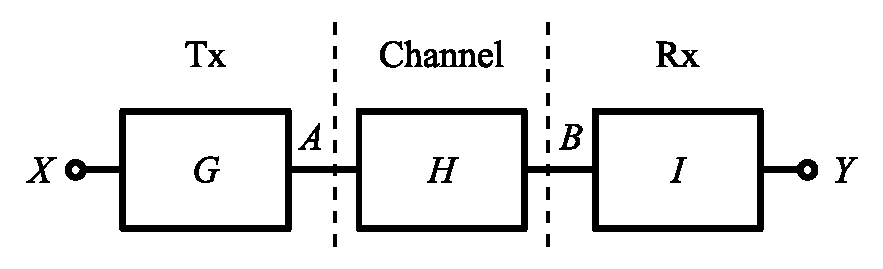
\includegraphics[scale=0.6]{TxRxEqualization}
	\caption{Channel equalization.}
\label{fig:TxRxEqualization}%##################################################
\end{figure}
%
\subsection{DFE Model}
\par The goal of the Rx equalizer will be to re-construct a time-delayed version of $X$ as the discrete-time binary signal, $Y$.
\begin{figure}[!ht]
	\centering
	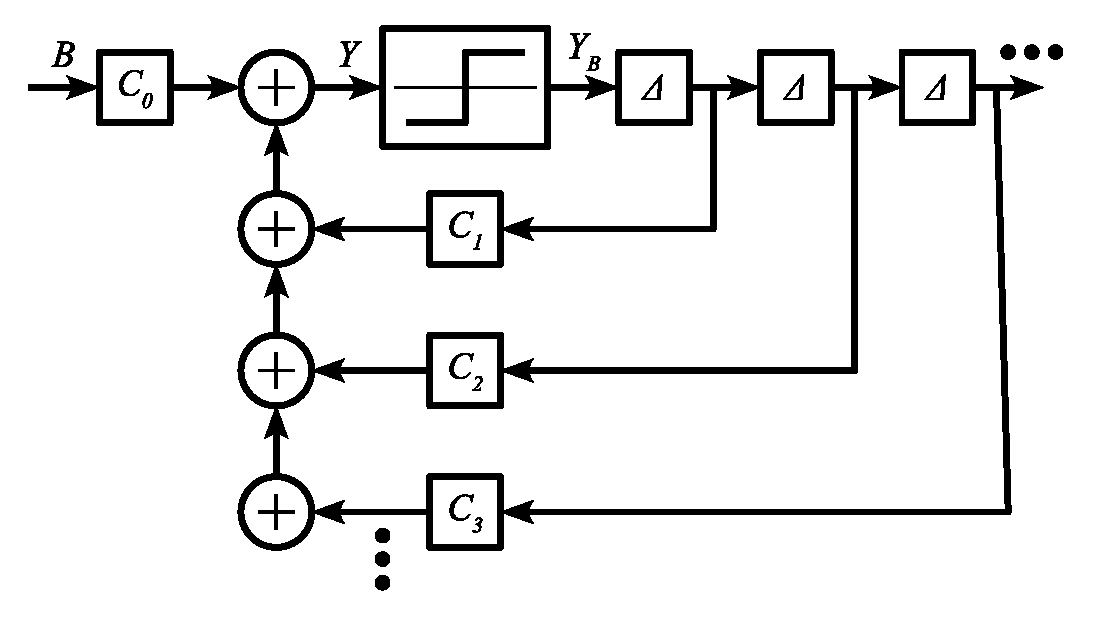
\includegraphics[scale=0.6]{DFEModel}
	\caption{DFE Model.}
\label{fig:DFEModel}%##################################################
\end{figure}
%
\par To achieve this goal, the DFE from Fig.~\ref{fig:DFEModel} will be used:
\begin{equation}
	Y_S=C_0 B + \sum\limits_{i=1}^{N}{C_i Y_L e^{-j\w(iT)}}.
\label{eq:DFE_Eq1}%##################################################
\end{equation}
%
\par For the simple case where the transmit filter $G$ is an ideal pulse generator, $P$:
\begin{equation}
	B=XPH
	\mathrm{.}
\label{eq:DFE_B_Expr1}%##################################################
\end{equation}
%
\begin{equation}
	P=
\begin{cases}
	1\mathrm{,} & 0\leq t \leq T
\\
	0\mathrm{,} & \textrm{otherwise.}
\end{cases}
\end{equation}
%
\par Break the loop: In an ideal world, the DFE would reconstruct the original signal before sampling it:
\begin{equation}
	Y_L = XP e^{-j\w (D-T)}
	\mathrm{.}
\label{eq:DFE_YL_Expr1}%##################################################
\end{equation}
where $D$ sets the sampling point right before the data is flopped.
%
\par Substituting \eqref{eq:DFE_B_Expr1}, and \eqref{eq:DFE_YL_Expr1} into \eqref{eq:DFE_Eq1}, the DFE can therefore be expressed as:
\begin{equation}
	Y_S=C_0 XPH + \sum\limits_{i=1}^{N}{C_i XP e^{-j\w(iT+D-T)}}.
\end{equation}
%
\begin{equation}
	\frac{Y_S}{X}=C_0 HP + P\sum\limits_{i=1}^{N}{C_i e^{-j\w(iT+D-T)}}.
\end{equation}
%
\subsection{Signal Sampling}
%-------------------------------------------------------------------------------
\begin{IEEEeqnarray}{rl}
	\symbSmplT(t, D) &{}\defAs \sum\limits_{-\infty}^{\infty}{\delta\brnd{t-(nT+D)}}
\\%##################################################
	\symbSmplT(t, D) &{}= \delta(t-D)\conv\sum\limits_{-\infty}^{\infty}{\delta\brnd{t-nT}}
\end{IEEEeqnarray}
\par Thus,
\begin{IEEEeqnarray}{rl}
	\symbSmplF(D) &{} \defAs \Fourier{\symbSmplT(t, D)}
\\%##################################################
	\symbSmplF(D) &{}= \frac{2\pi e^{-j\w D}}{T}\sum\limits_{k=-\infty}^{\infty}{\delta\brnd{\w-\frac{2\pi k}{T}}}
\end{IEEEeqnarray}
%
\subsection{Amplitude Equalization}
%-------------------------------------------------------------------------------
\begin{IEEEeqnarray}{rll}
	\frac{Y_S}{X} &{}= e^{-j\w D}\mathrm{,}
	&{}\quad\forall t=iT+D
\\%##################################################
	e^{-j\w D} &{}= C_0 HP + P\sum\limits_{i=1}^{N}{C_i e^{-j\w(iT+D-T)}}\mathrm{,}
	&{}\quad\forall t=iT+D
\end{IEEEeqnarray}
%
\par Part 1, $t=D$:
\begin{IEEEeqnarray}{rll}
	e^{-j\w D} &{}= C_0 HP\mathrm{,}
	&{}\quad t=D
\\%##################################################
	\delta(t-D) &{}= C_0 h_P(t)
	&{}\quad t=D
\\%##################################################
	C_0 &{}= 1/h_P(D)
	&{}
\end{IEEEeqnarray}
%
\par Part 2, $t=iT+D\quad i>0$:
\begin{IEEEeqnarray}{rll}
	P\sum\limits_{i=1}^{N}{C_i e^{-j\w(iT+D-T)}} &{}= e^{-j\w D} - C_0 HP\mathrm{,}
	&{}\quad t=iT+D\quad i>0
\\%##################################################
	P \sum\limits_{i=1}^{N}{C_i e^{-j\w(iT+D-T)}} &{}= e^{-j\w D} - C_0 HP\mathrm{,}
	&{}\quad t=iT+D\quad i>0
\end{IEEEeqnarray}
%
\par If we want to use arbitrary filter $F$ with feedback coefficients:
\begin{equation}
	C_i\Rightarrow F C_i\mathrm{,}\quad i>0.
\end{equation}
%
\par Thus we get
\begin{IEEEeqnarray}{rll}
	P\sum\limits_{i=1}^{N}{C_i e^{-j\w(iT+D-T)}} &{}= \frac{e^{-j\w D} - C_0 HP}{F}\mathrm{,}
	&{}\quad t=iT+D\quad i>0
%\\%##################################################
\end{IEEEeqnarray}
%
\section{Matrix Test}
%-------------------------------------------------------------------------------
\begin{IEEEeqnarray}{rl}
	\matrixsymbol{V}&{}=\matrixsymbol{ZI}
\label{eq:ZPMatrixEquation}\\%##################################################
	\nRowColMx{V}{}{N}&{}=\nXnMx{z}{}{n}{n}\nRowColMx{I}{}{N}
	\textrm{.}
\end{IEEEeqnarray}
%Last line
%
%\input{_Test}%
%
\backmatter%Supposed to be called before the bibliography & index - I don't know why
%------------------------------------------------------------------------------
%Bibliography
%------------------------------------------------------------------------------
\bibliographystyle{IEEEtran}%
\cleardoublepage%Go to next page so that "\addcontentsline" points to the correct page
	\addcontentsline{toc}{chapter}{\bibname}%Add bibliography to table of contents
	\bibliography{IEEEfull,../Common/CustomStrings,../Common/ReferenceDB}%
%
\end{document}%
%Last line
